\documentclass{beamer}
\usepackage{url}
\usepackage{color}

\title{Quick Intro to Git version control}
%\author{Alexandre Beaulne}

\begin{document}

\begin{frame}
    \titlepage
\end{frame}

\begin{frame}
    \frametitle{Contents}
    \tableofcontents[hideallsubsections]
\end{frame}

\section{Intro}

\begin{frame}
    \frametitle{Intro}
    \begin{center}
        Git is an open source, \textbf{distributed} version control
        system designed for speed and efficiency.
    \end{center}
\end{frame}

\begin{frame}
    \frametitle{Centralized paradigm (CVS, SVN, Perforce)}
    \begin{figure}[h!]
        \begin{center}
            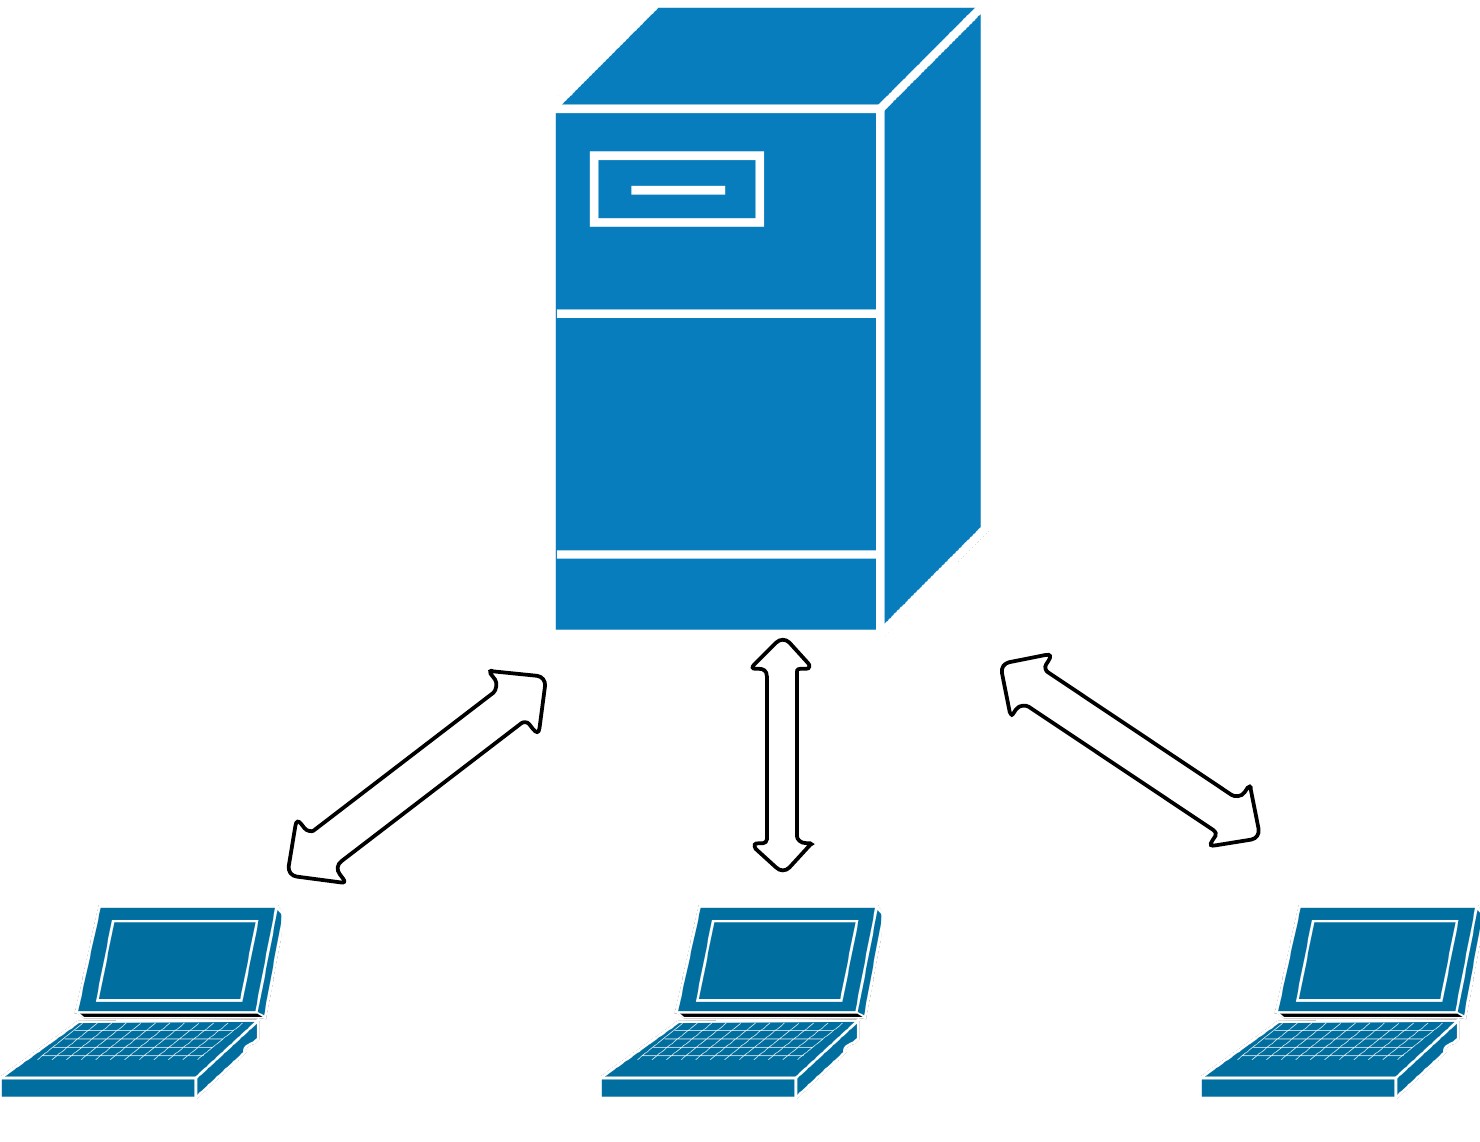
\includegraphics[scale=0.175]{centralized.png}
        \end{center}
    \end{figure}
\end{frame}

\begin{frame}
    \frametitle{Distributed paradigm (Git, Mercurial)}
    \begin{figure}[h!]
        \begin{center}
            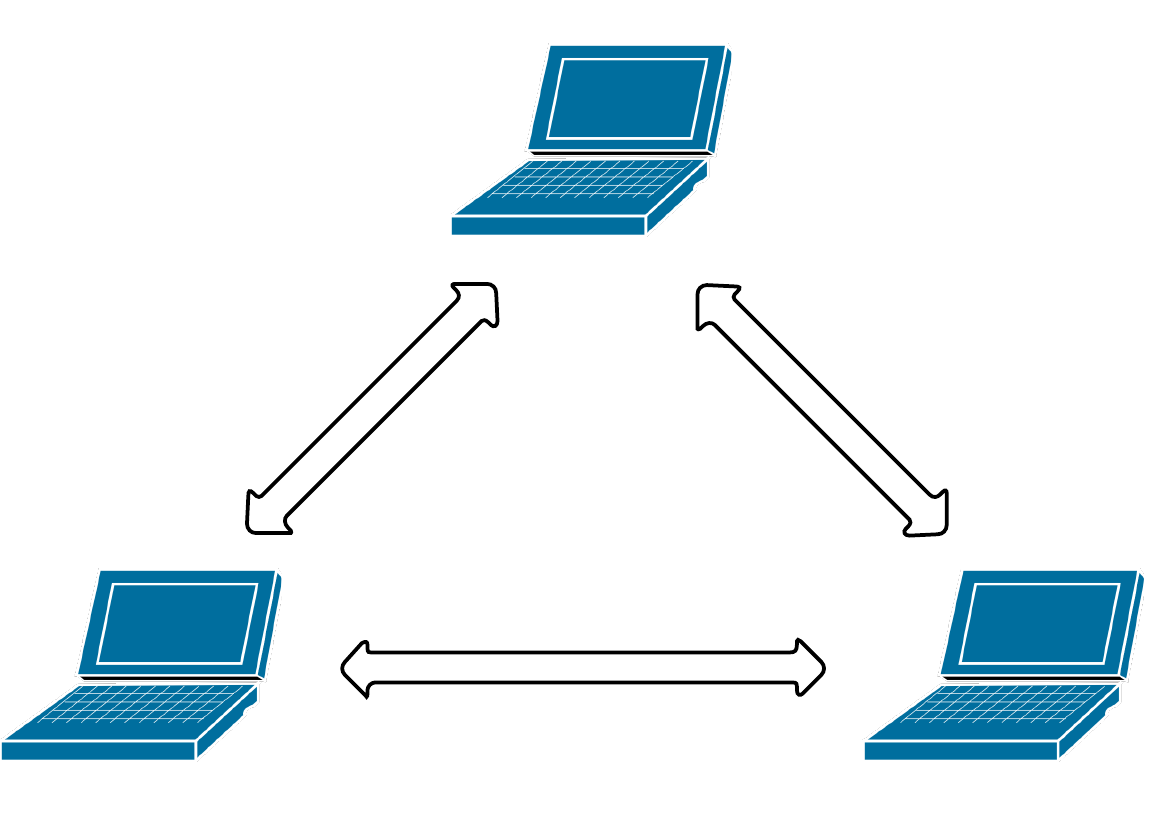
\includegraphics[scale=0.55]{distributed.png}
        \end{center}
    \end{figure}
\end{frame}

\section{Commands}

\begin{frame}
    \frametitle{Git commands}
    \begin{figure}[h!]
        \begin{center}
            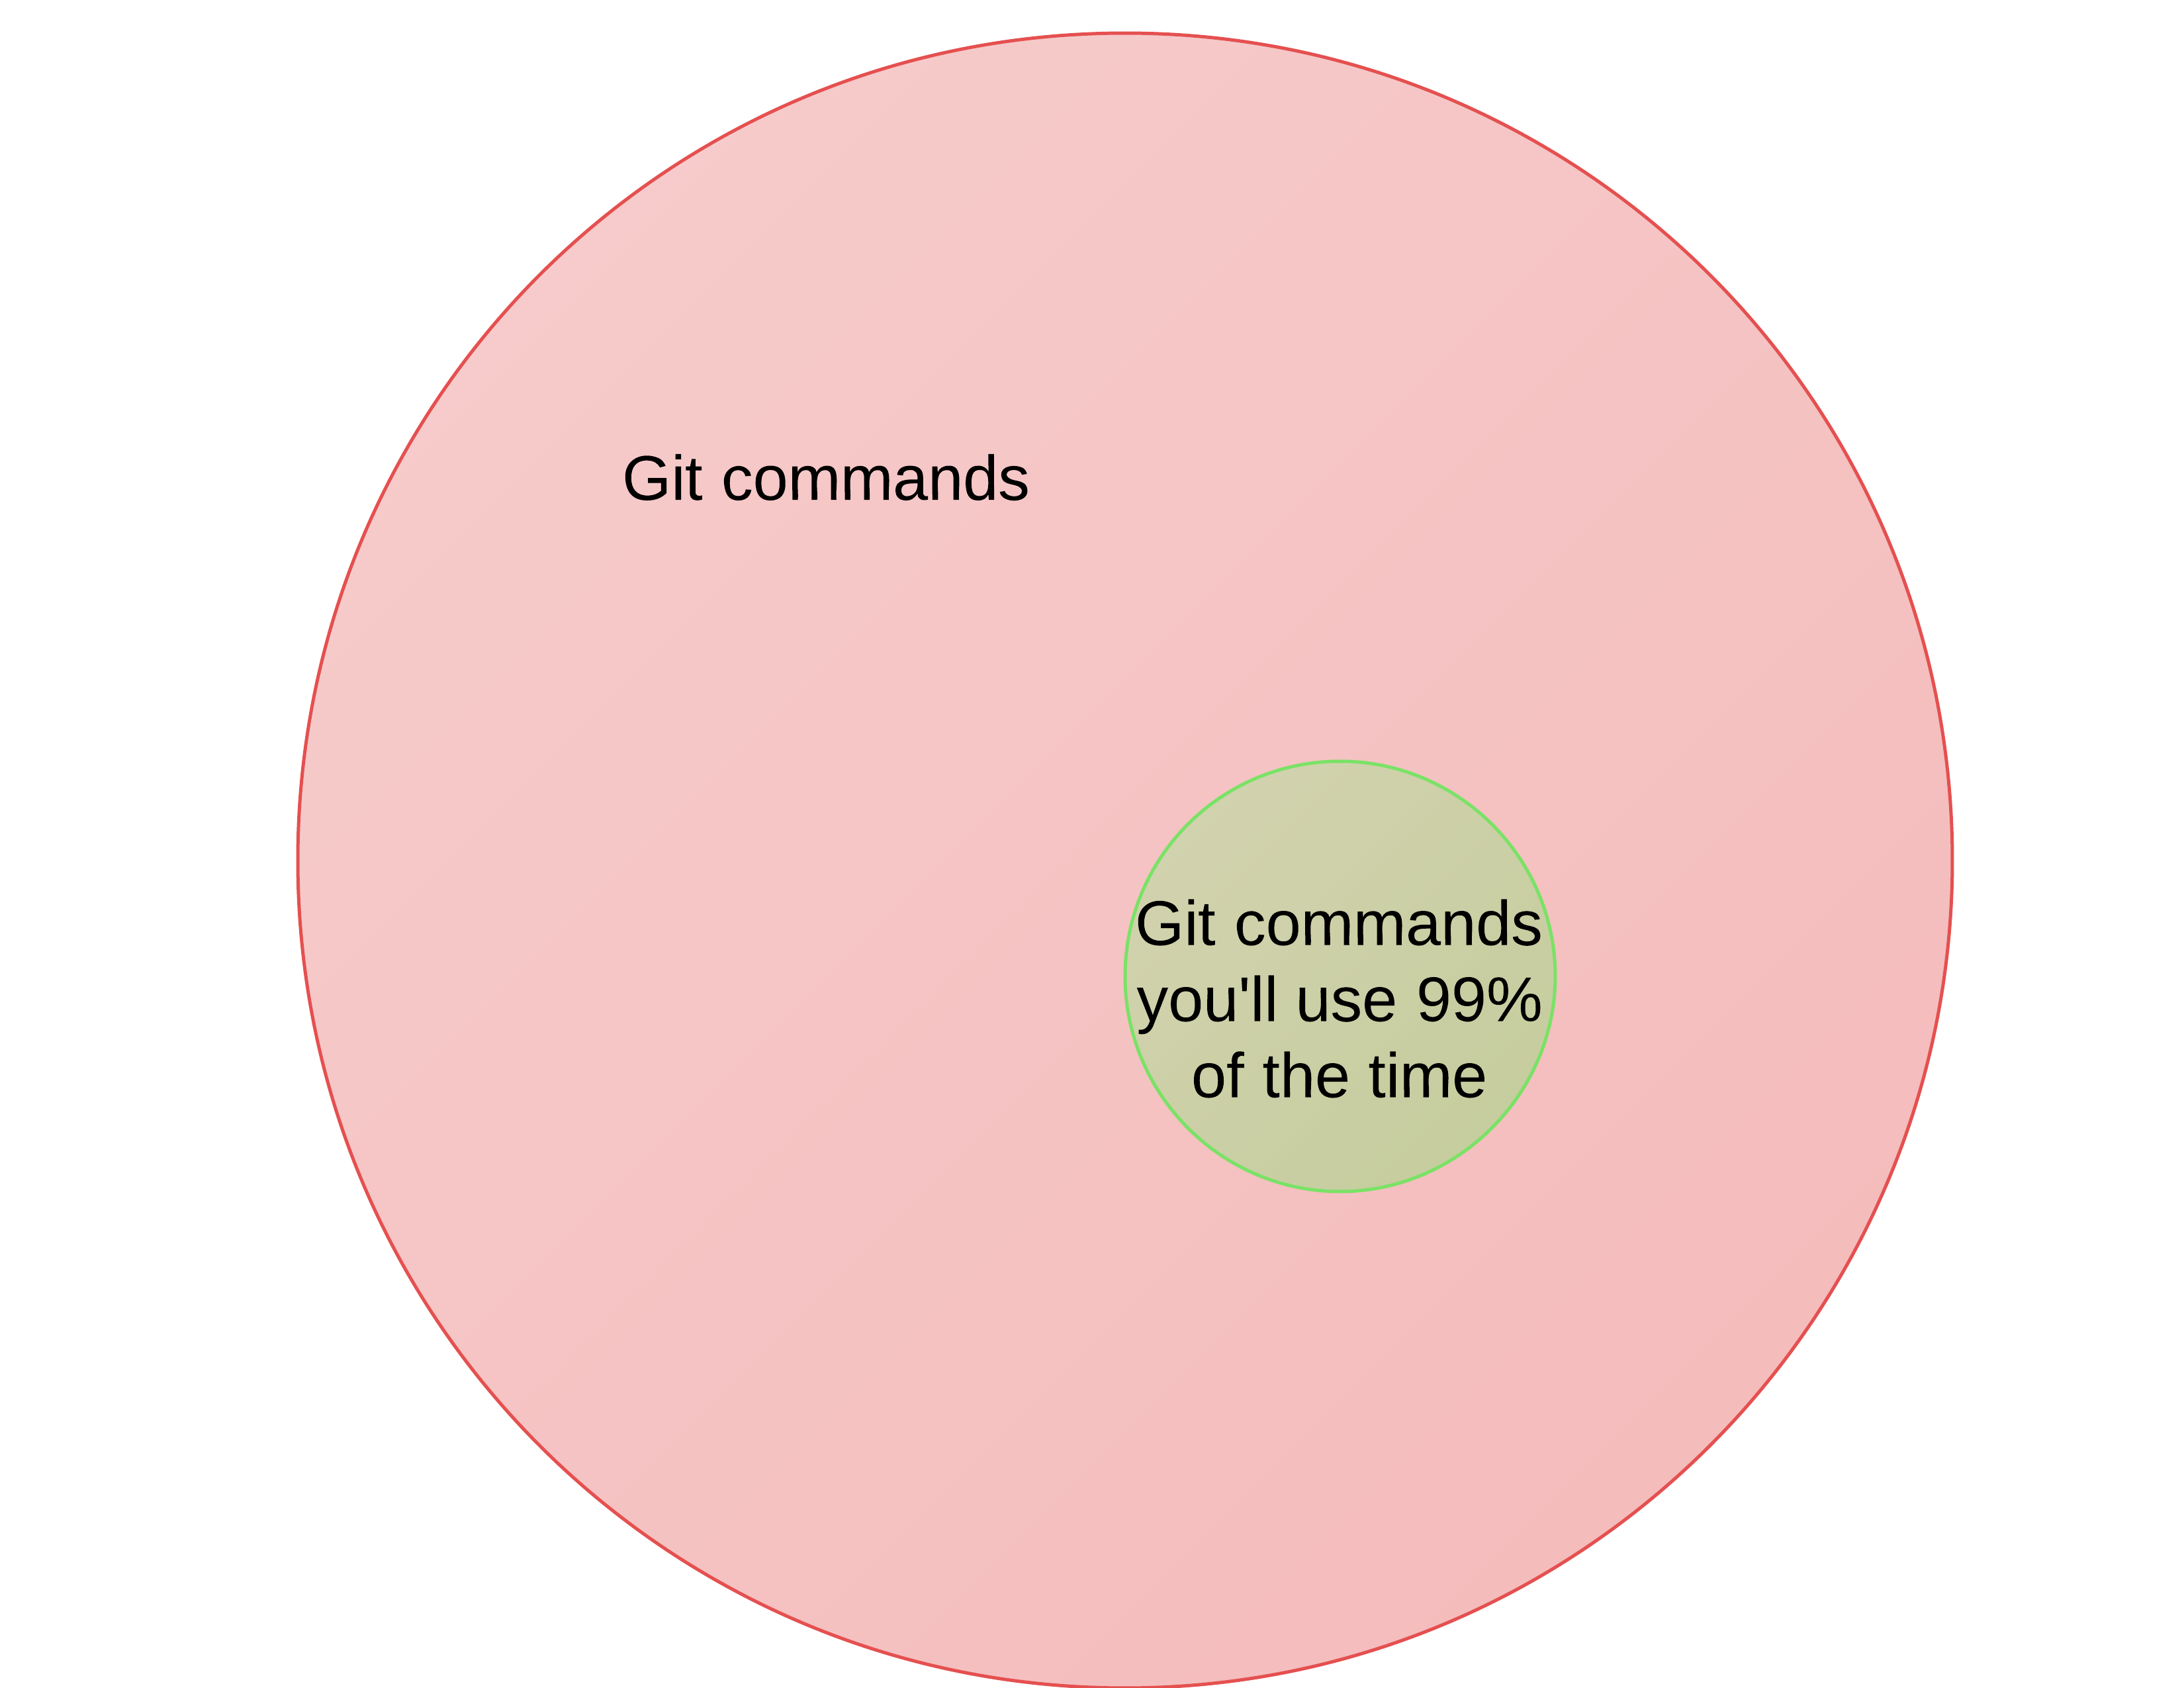
\includegraphics[scale=0.09]{git_commands1.png}
        \end{center} \end{figure}
\end{frame}

\begin{frame}
    \frametitle{Git commands}
    \begin{figure}[h!]
        \begin{center}
            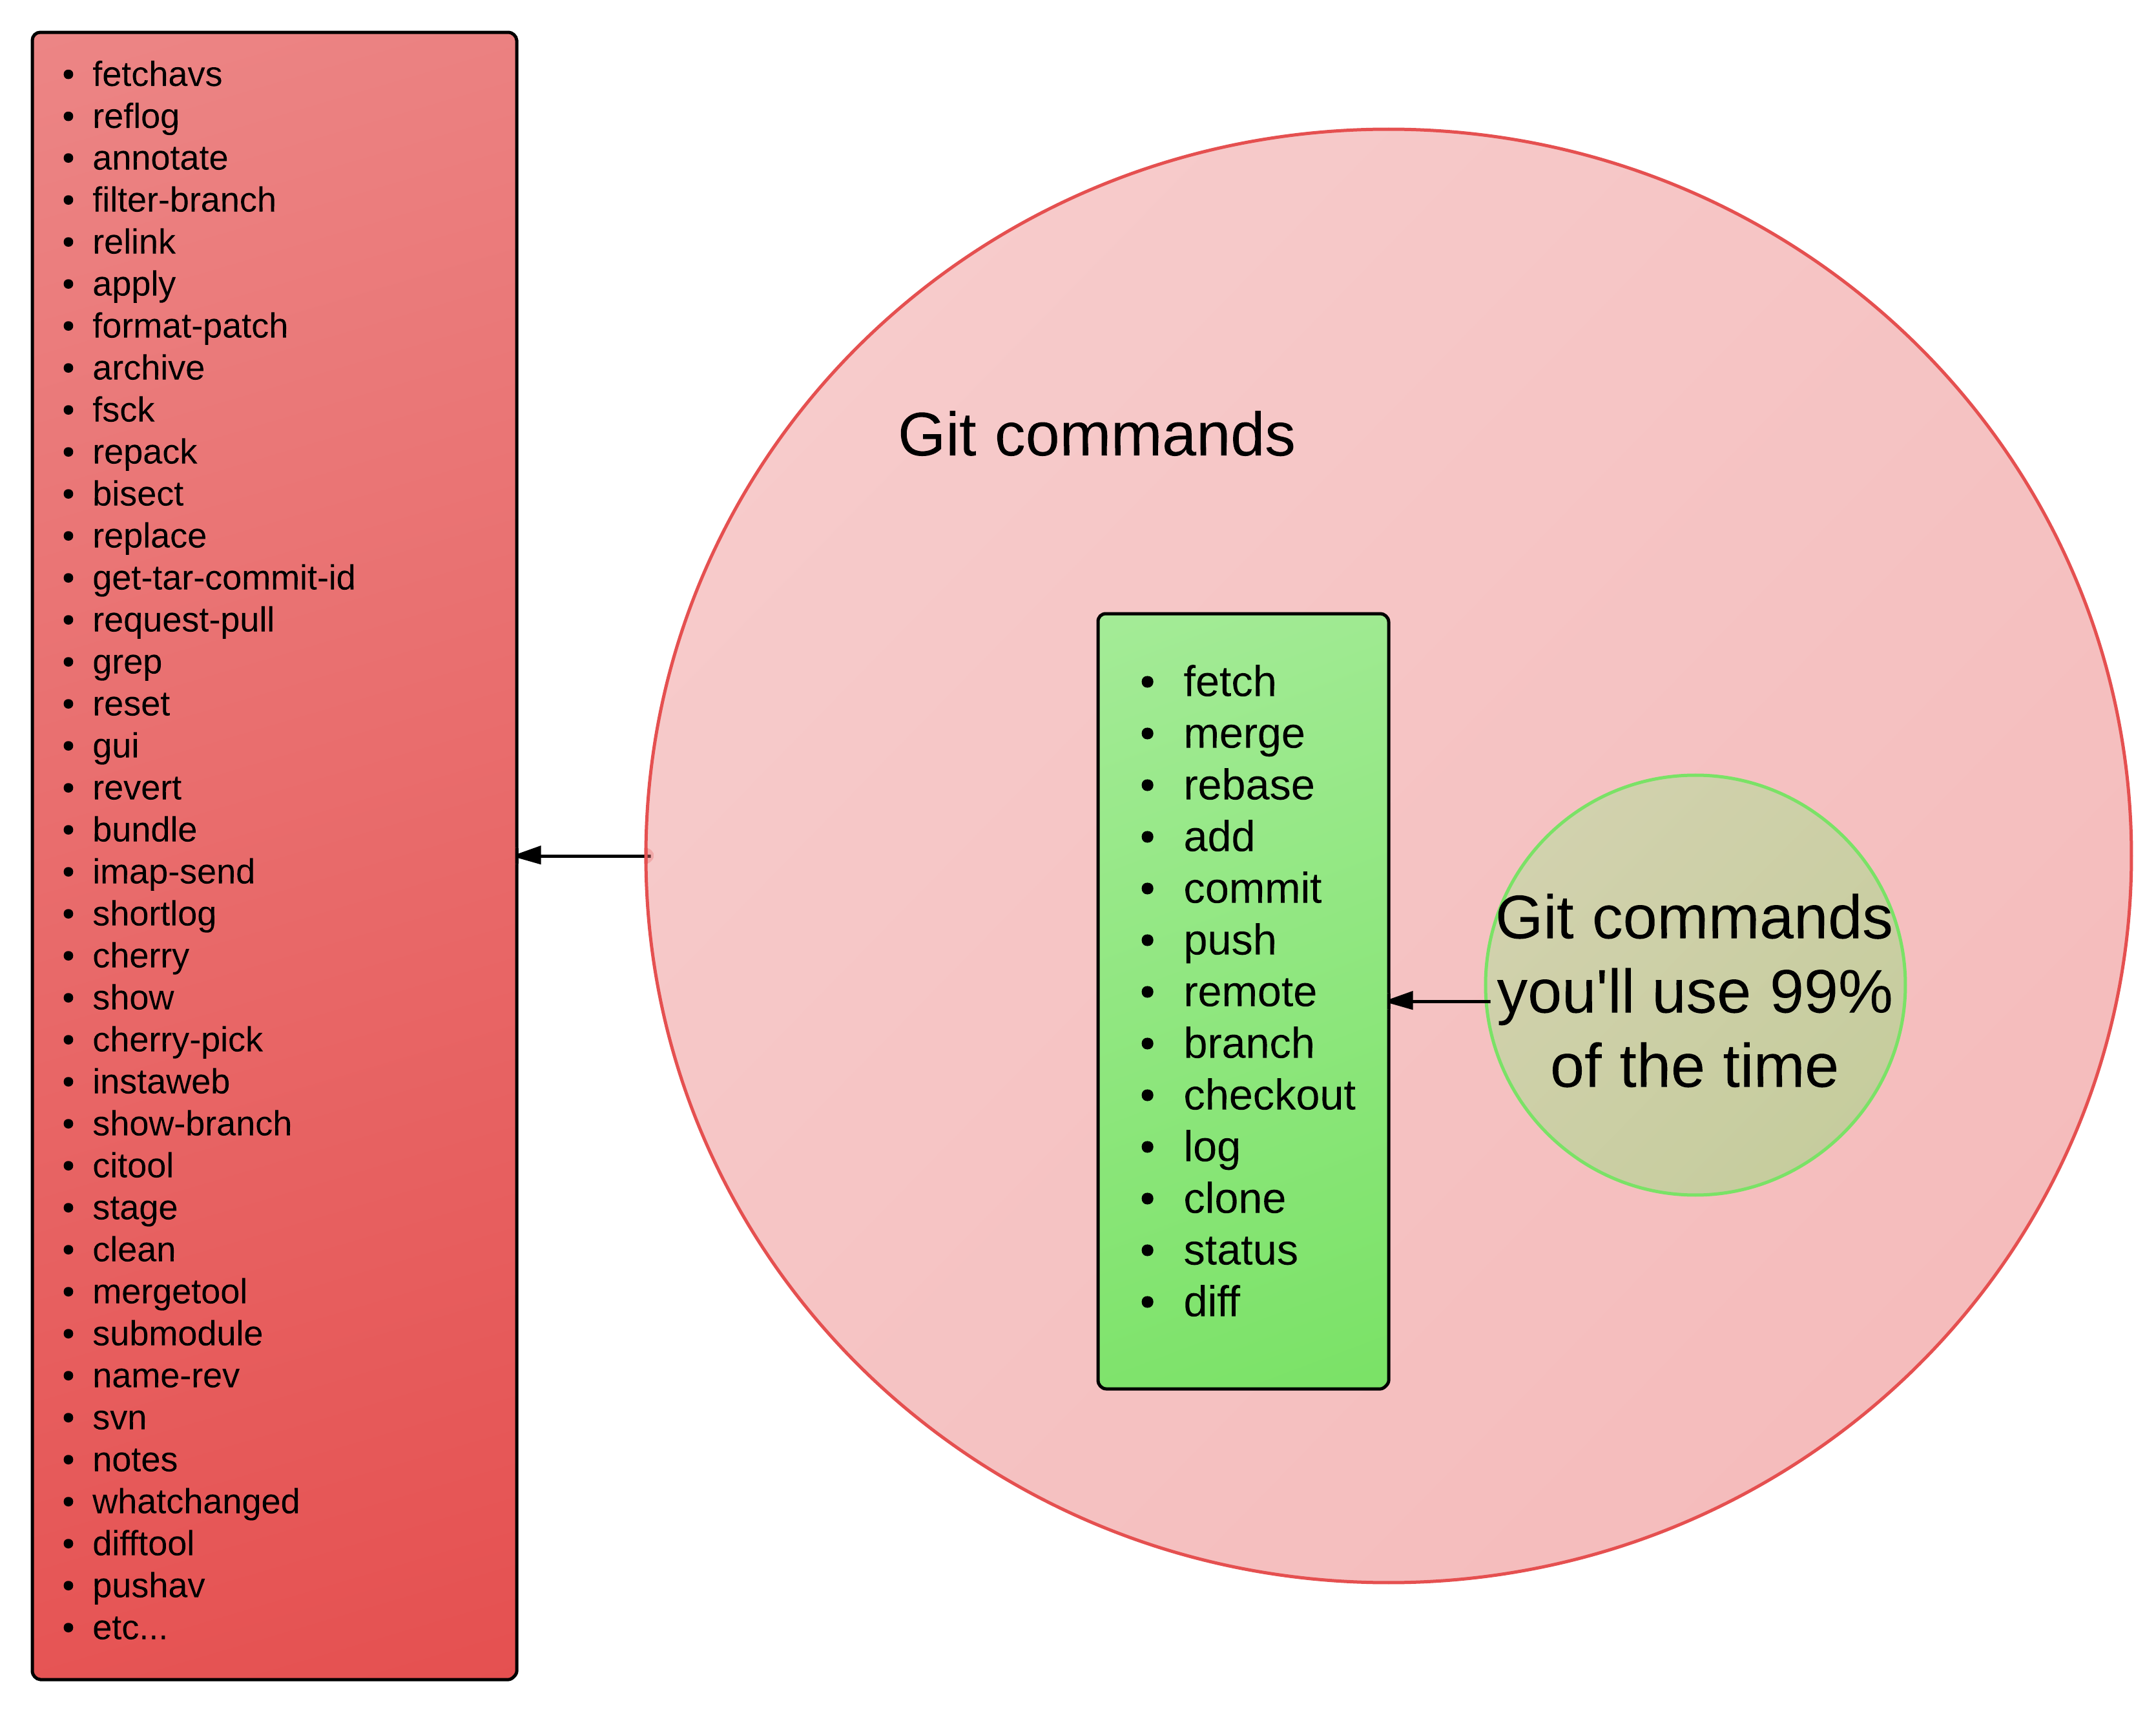
\includegraphics[scale=0.09]{git_commands2.png}
        \end{center}
    \end{figure}
\end{frame}

\begin{frame}
    \frametitle{Git commands}
    \begin{figure}[h!]
        \begin{center}
            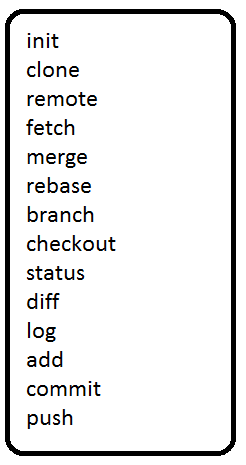
\includegraphics[scale=0.6]{commands.png}
        \end{center}
    \end{figure}
\end{frame}

\subsection{IDEs}

\begin{frame}
    \frametitle{Eclipse}
    \begin{figure}[h!]
        \begin{center}
            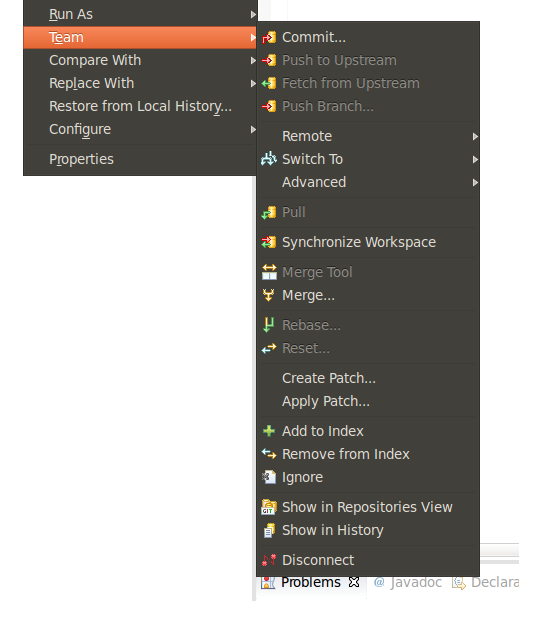
\includegraphics[scale=0.55]{eclipse1.png}
        \end{center}
    \end{figure}
\end{frame}

\begin{frame}
    \frametitle{Eclipse}
    \begin{figure}[h!]
        \begin{center}
            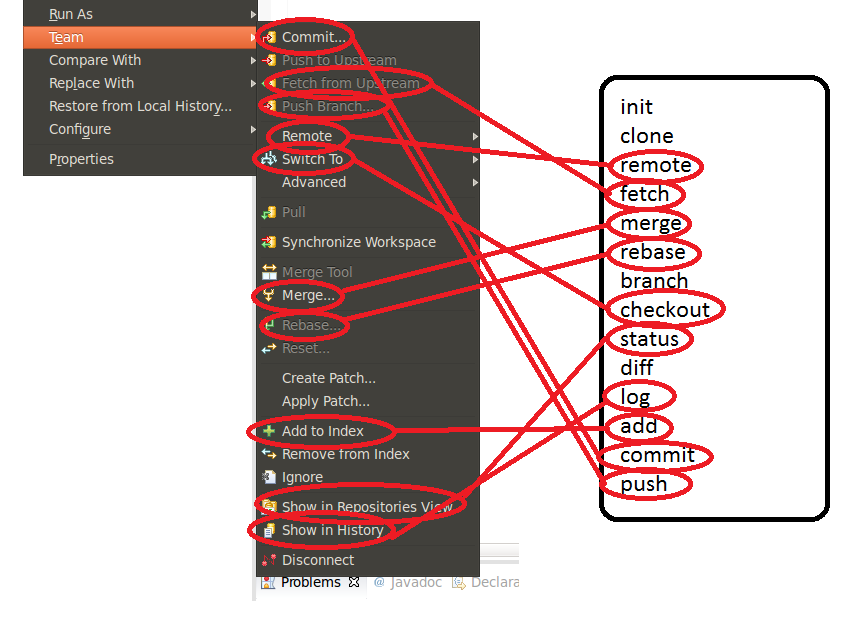
\includegraphics[scale=0.5]{eclipse2.png}
        \end{center}
    \end{figure}
\end{frame}

\begin{frame}
    \frametitle{IntelliJ}
    \begin{figure}[h!]
        \begin{center}
            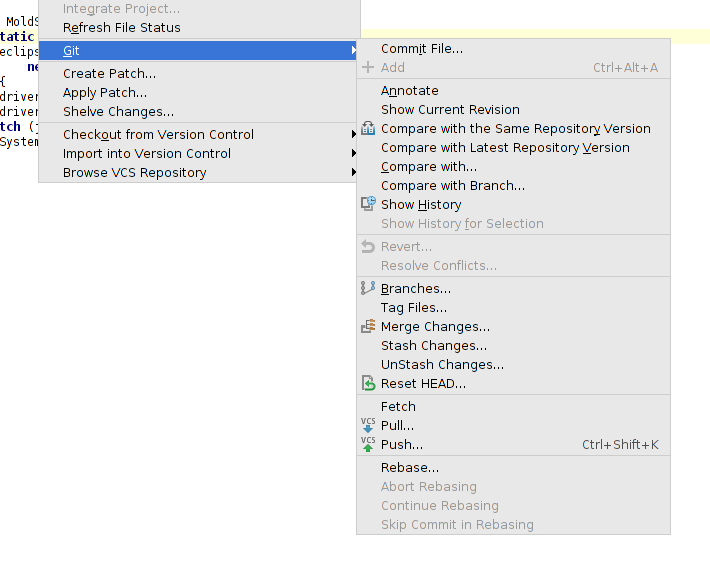
\includegraphics[scale=0.55]{intellij1.png}
        \end{center}
    \end{figure}
\end{frame}

\begin{frame}
    \frametitle{IntelliJ}
    \begin{figure}[h!]
        \begin{center}
            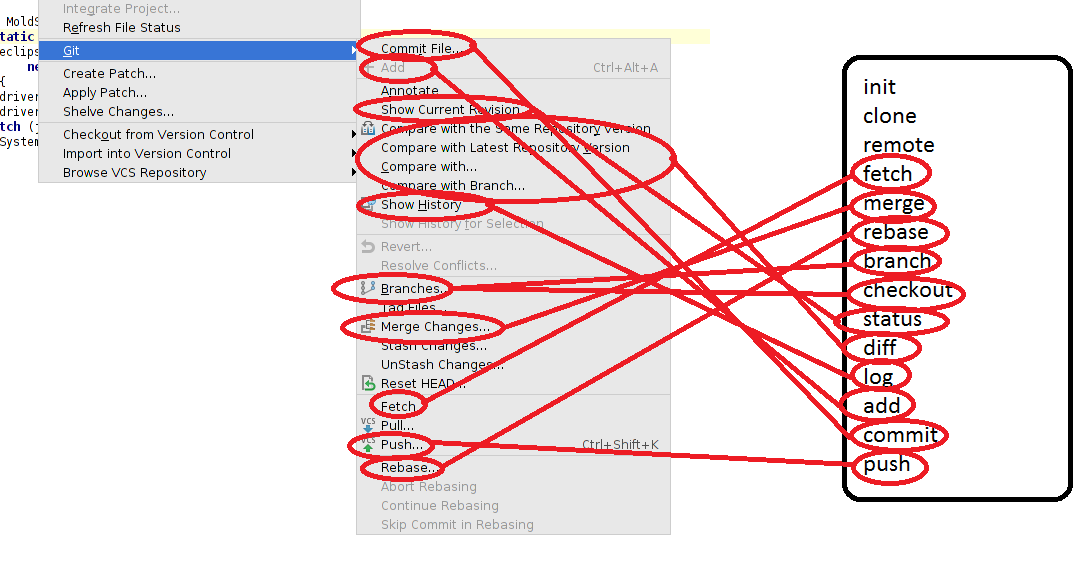
\includegraphics[scale=0.4]{intellij2.png}
        \end{center}
    \end{figure}
\end{frame}

\begin{frame}[fragile]
    \frametitle{\$ git config}
    \begin{figure}[h!]
        \begin{center}
            
\includegraphics[scale=0.7]{config.png}
        \end{center}
    \end{figure}
    \begin{verbatim}
$ git config --global user.email abeaulne@eclipseoptions.com
$ git config --global user.name 'Alex Beaulne'
    \end{verbatim}
    is necessary to get started. \textbf{Use short email for proper integration with Stash}
\end{frame}

\begin{frame}[fragile]
    \frametitle{\$ git init}
    \begin{figure}[h!]
        \begin{center}
            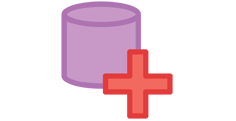
\includegraphics[scale=0.7]{init.png}
        \end{center}
    \end{figure}
    \begin{verbatim}
$ git init
    \end{verbatim}
    makes the current working directory a Git repository
\end{frame}

\begin{frame}
    \frametitle{\$ git init}
    \begin{figure}[h!]
        \begin{center}
            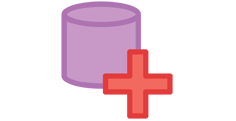
\includegraphics[scale=0.7]{init.png}
        \end{center}
    \end{figure}
    a hidden directory .git is inserted in the root directory
    of the Git repository. Unlike CVS or SVN, no .git directory
    is inserted in each subdirectories
\end{frame}

\begin{frame}
    \frametitle{\$ git remote}
    \begin{figure}[h!]
        \begin{center}
            
\includegraphics[scale=0.7]{remote.png}
        \end{center}
    \end{figure}
    A Git remote is best thought as an alias for a URL.
    It's an address to a remote Git repository from
    which you can fetch or push source code.
\end{frame}

\begin{frame}[fragile]
    \frametitle{\$ git remote}
    \begin{figure}[h!]
        \begin{center}
            
\includegraphics[scale=0.7]{remote.png}
        \end{center}
    \end{figure}
    Create a new remote:
    \begin{verbatim}
    $ git remote add remote_name remote_url
    \end{verbatim}
    List remotes:
    \begin{verbatim}
    $ git remote -v
    \end{verbatim}
\end{frame}

\begin{frame}[fragile]
    \frametitle{\$ git clone}
    \begin{figure}[h!]
        \begin{center}
            
\includegraphics[scale=0.7]{clone.png}
        \end{center}
    \end{figure}
    \begin{verbatim}
$ git clone remote_url
    \end{verbatim}
    create a local copy of the Git repository hosted at remote\_url
\end{frame}

\begin{frame}[fragile]
    \frametitle{\$ git status}
    \begin{figure}[h!]
        \begin{center}
            
\includegraphics[scale=0.7]{status.png}
        \end{center}
    \end{figure}
    \begin{verbatim}
$ git status
    \end{verbatim}
    shows which files on the current branch are untracked, modified and staged for commit
\end{frame}

\begin{frame}[fragile]
    \frametitle{\$ git pull}
    \begin{figure}[h!]
        \begin{center}
            
\includegraphics[scale=0.7]{pull.png}
        \end{center}
    \end{figure}
    \begin{verbatim}
$ git pull remote_name_or_url branch_name
    \end{verbatim}
    apply new commits from the remote Git repository to the local repository
\end{frame}

\begin{frame}[fragile]
    \frametitle{\$ git branch}
    \begin{figure}[h!]
        \begin{center}
            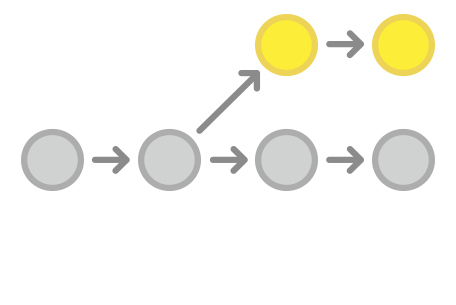
\includegraphics[scale=0.4]{branch.png}
        \end{center}
    \end{figure}
    \begin{verbatim}
$ git branch new_branch_name
    \end{verbatim}
    is used to create a new branch from the current branch
\end{frame}

\begin{frame}[fragile]
    \frametitle{\$ git branch}
    Without a branch name, it will list all the branch in the local repository:
    \begin{verbatim}
$ git branch
  develop
* featureJIRA12
  master
    \end{verbatim}
the asterisk shows the current branch
\end{frame}

\begin{frame}[fragile]
    \frametitle{\$ git checkout}
    \begin{figure}[h!]
        \begin{center}
            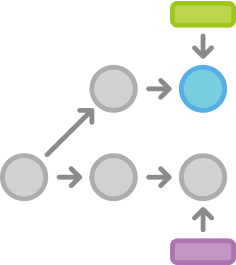
\includegraphics[scale=0.5]{checkout.png}
        \end{center}
    \end{figure}
    \begin{verbatim}
$ git checkout branch_name
    \end{verbatim}
    is used to switch between branches
\end{frame}

\begin{frame}[fragile]
    \frametitle{\$ git diff}
    \begin{figure}[h!]
        \begin{center}
            
\includegraphics[scale=1.2]{diff.png}
        \end{center}
    \end{figure}
    \begin{verbatim}
$ git diff [filename1 [filename2]...]
    \end{verbatim}
    shows lines that have changed since latest commit on branch
\end{frame}

\begin{frame}[fragile]
    \frametitle{\$ git diff}
    \begin{figure}[h!]
        \begin{center}
            
\includegraphics[scale=1.2]{diff.png}
        \end{center}
    \end{figure}
    \begin{verbatim}
$ git diff [filename1 [filename2]...]
    \end{verbatim}
    If no file is specified, show diff for all modified files on the current branch
\end{frame}

\begin{frame}
    \frametitle{two notes on Git commits}
    I. A Git commit is `repository-wide'. It is a snapshot
    of the complete repository at that point in time. This
    is different to CVS per-file commits.
\end{frame}

\begin{frame}
    \frametitle{two notes on Git commits}
    II. Pushing a commit to a canonical Git repository
    is a three stages process: (i) add (ii) commit (iii) push.
    Unlike CVS, a Git commit does not push anything to a remote
    repository. One needs to push to do so.
\end{frame}

\begin{frame}[fragile]
    \frametitle{\$ git add}
    \begin{figure}[h!]
        \begin{center}
            
\includegraphics[scale=0.7]{add.png}
        \end{center}
    \end{figure}
    \begin{verbatim}
$ git add [filename1 [filename2]...]
    \end{verbatim}
    is used to add files to staging area
\end{frame}

\begin{frame}[fragile]
    \frametitle{\$ git commit}
    \begin{figure}[h!]
        \begin{center}
            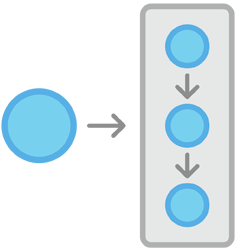
\includegraphics[scale=0.7]{commit.png}
        \end{center}
    \end{figure}
    \begin{verbatim}
$ git commit -m "commit msg JIRA-XXX"
    \end{verbatim}
    commits the changes previously added to staging area
\end{frame}

\begin{frame}[fragile]
    \frametitle{\$ git log}
    \begin{figure}[h!]
        \begin{center}
            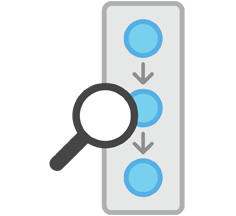
\includegraphics[scale=0.7]{log.png}
        \end{center}
    \end{figure}
    \begin{verbatim}
$ git log [-n] [branch_name]
    \end{verbatim}
    shows latest n (or all) commits for branch 'branch\_name' (default to current branch)
\end{frame}

\begin{frame}[fragile]
    \frametitle{\$ git push}
    \begin{figure}[h!]
        \begin{center}
            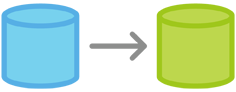
\includegraphics[scale=0.7]{push.png}
        \end{center}
    \end{figure}
    \begin{verbatim}
$ git push remote_name_or_url branch_name
    \end{verbatim}
    pushes local commits to remote branch
\end{frame}

\section{Workflow}

\begin{frame}
    \frametitle{Workflows}
    \begin{itemize}
        \item Centralized workflow
        \item Feature branch workflow
        \item Gitflow workflow
        \item Forking workflow
    \end{itemize}
\end{frame}

\begin{frame}
    \frametitle{Workflows}
    \begin{itemize}
        \item \textcolor{gray}{Centralized workflow}
        \item \textcolor{gray}{Feature branch workflow}
        \item Gitflow workflow
        \item \textcolor{gray}{Forking workflow}
    \end{itemize}
\end{frame}

\begin{frame}
    \frametitle{Gitflow}
    \begin{figure}[h!]
        \begin{center}
            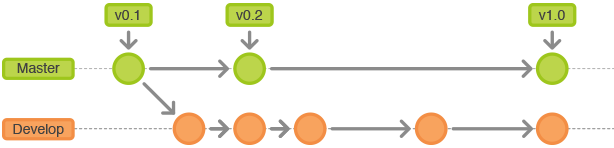
\includegraphics[scale=0.5]{gitflow2.png}
        \end{center}
    \end{figure}
\end{frame}

\begin{frame}
    \frametitle{Gitflow}
    \begin{figure}[h!]
        \begin{center}
            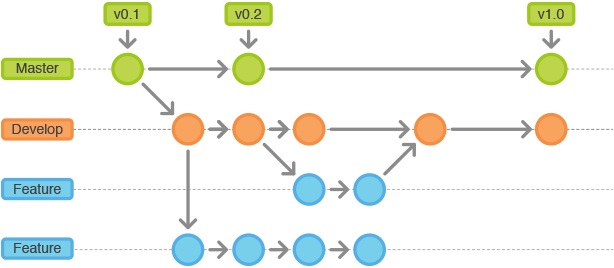
\includegraphics[scale=0.5]{gitflow3.png}
        \end{center}
    \end{figure}
\end{frame}

\begin{frame}
    \frametitle{Gitflow}
    \begin{description}
      \item[master branch] stores the official release history. It is only changed when the Bamboo
          users merge the develop branch into it
      \item[develop branch] serves as an integration branch for features. It is only changed when
          feature branches are merged into it (via pull request, no direct push)
      \item[feature branches] are where new features reside. Features branches are branched from
          the develop branch, and their changes are incorporated in the canonical repo via pull
          requests to the develop branch
    \end{description}
\end{frame}

\section{Pull requests}

\begin{frame}
    \frametitle{Pull requests}
    \begin{itemize}
        \item Not part of Git per se
        \item More a feature of Git hosting solutions (Stash, Github, etc)
        \item Great for code reviews
    \end{itemize}
\end{frame}

\begin{frame}
    \frametitle{Pull requests}
    demo
\end{frame}

\section{Resources}

\begin{frame}
    \frametitle{Resources}
    \begin{itemize}
        \item These slides are on Confluence (\url{http://confluence/display/~abeaulne/Intro+to+Git+presentation})
        \item More detailed instructions Trading Systems team at \url{http://confluence/display/TSD/Setting+up+GIT}
        \item Atlassian has a great straightforward tutorial at \url{https://www.atlassian.com/git/}
    \end{itemize}
\end{frame}

\section{Homework}

\begin{frame}
    \frametitle{Homework}
    \begin{itemize}
        \item fetch canonical `practice' repository at \url{http://stash/scm/core/practice.git}
        \item create a feature branch (branched out of develop branch) with your name
        \item add your name to the README.txt
        \item commit your change locally
        \item push your commit to remote feature branch at canonical `practice' repo
        \item create a pull request, adding me (Alex) and one of your colleagues/superiors as reviewer
    \end{itemize}
\end{frame}

\begin{frame}[fragile]
    \frametitle{Solution}
    \begin{verbatim}
~$ git clone http://stash/scm/core/practice.git
~$ cd practice/
~/practice$ git checkout develop
~/practice$ git branch alexb
~/practice$ git checkout alexb
~/practice$ vim README.txt
~/practice$ git add README.txt
~/practice$ git commit -m "added my name"
~/practice$ git push origin alexb
    \end{verbatim}
    Finally go to \url{http://stash/projects/CORE/repos/practice/browse} to create pull request
\end{frame}

\end{document}

